\documentclass{iopjournal}
\usepackage{amsmath,amssymb,amsfonts}%
\usepackage{amsthm}%
\usepackage{mathrsfs}%
\usepackage{booktabs}%
\usepackage{xcolor}%
\usepackage{listings}%
\usepackage{wasysym}%
\usepackage{textcomp}%
\usepackage{manyfoot}%
\usepackage[title]{appendix}%
\usepackage{algorithm}%
\usepackage{algorithmicx}%
\usepackage{algpseudocode}%
\usepackage{enumitem}%
\usepackage[
    backend=biber,
    style=numeric,
]{biblatex}%
\addbibresource{./citations.bib}

% Options
	% [anonymous]	Provides output without author names, affiliations or acknowledgments to facilitate double-anonymous peer-review

\begin{document}

\articletype{Paper}%	 e.g. Paper, Letter, Topical Review...

\title{Relativity without a Time Dimension: Absolute Time, Co-expansion, and a Departure from General Relativity at Second Order}

\author{Andrew Mueller$^1$\orcid{0000-0003-0573-6327}}

\affil{$^1$Independent Researcher, Milwaukee, USA}

\email{AndrewMueller414@gmail.com}

\keywords{gravitation, time, relativity, equivalence principle, Kaluza--Klein theory, Painlev\'e--Gullstrand coordinates, preferred frame}

\begin{abstract}
Special relativity is normally written with time as a fourth dimension. We show that its kinematics can instead be written with a fourth spatial axis $y$ and no time dimension. Motion along the four axes is the fundamental rate of change, and the inclination of a body's path into $y$ carries the kinematics: its slope is $\beta\gamma$, its sine is the speed, and its cosine is the rate of a clock carried along it. Time is a ratio of distances, light enters only as a causal sphere, and every inertial observer recovers one absolute time. Gravity uses the same inclination and one further postulate: all matter co-expands with the change in $y$, every length by the local Lorentz factor and every clock by its inverse. The universality of this co-expansion is the origin of the equivalence principle. With space flowing outward from every mass, the Lorentz factor obeys a linear field equation outside matter. The geometry agrees with general relativity at first post-Newtonian order, including perihelion advance, light bending and Shapiro delay. It differs beyond that order: second-order light deflection is larger, and the horizon is the absolute centre.
\end{abstract}

\section{Introduction}\label{sec1}

In special relativity time is a fourth dimension of spacetime, and its rate is tied to the speed of light. Time does two jobs there: it locates events, as a fourth coordinate does, and it orders change, as a rate does. This paper keeps both jobs and removes time as a dimension. The fourth coordinate becomes a spatial one, a density axis $y$ that extends ordinary space $\mathbb{R}^3$ in the manner of an unwrapped, non-compact Kaluza--Klein dimension~\cite{Kaluza1921, Klein1926}. The rate of change becomes motion, which is primitive and is not measured against anything else. A body moves along four axes: the three of $\mathbb{R}^3$ and the density axis, along which it is carried by its own motion.

One geometric object carries the argument: the inclination of a path through $\mathbb{R}^3\times y$. Section~\ref{sec_motion} shows that it contains the kinematics of special relativity (SR)~\cite{einstein1905electrodynamics}. Its slope is $\partial_x y=\beta\gamma$, so that $\gamma=\sqrt{1+(\partial_x y)^2}$; its sine is the speed; and its cosine is the coordinate density, which is also the rate of a clock carried along the path. Time readings are ratios of distances along the path, and the speed of light enters only as the speed of the causal sphere that spreads from each event. Every inertial observer can then recover one absolute time, and the relativity of simultaneity becomes a displacement along $y$.

Section~\ref{sec_gravity} builds gravity from the same inclination and one postulate, co-expansion: all matter co-expands with the change in $y$, every material length by the local Lorentz factor $\gamma$ and every clock by $1/\gamma$. Because the rescaling is the same for all matter, free fall cannot depend on composition, and the equivalence principle follows from the geometry. Space is taken to flow outward from every mass, as in the Hubble flow, at the speed $\beta c$ with $\beta^2=2GM/(c^2R)$. Co-expansion fixes which radius sets the flow: the source has itself co-expanded, so $R$ is its measured radius, $\gamma$ times its absolute radius. This fixes $\gamma$ self-consistently, and the rule is the point-mass solution of a linear field equation for $\gamma-1/\gamma$ in flat absolute space. The resulting space is inclined into $y$ exactly as a moving path is, its height is the offset between absolute and static clocks, and light and matter move through flat absolute space with no time coordinate (section~\ref{sec_time_elimination}). Section~\ref{sec_kk} places the density axis in a five-dimensional Kaluza--Klein metric. Section~\ref{sec_gamma_coscaling} lists where the geometry agrees with general relativity and where it does not, and section~\ref{sec_discussion} states what has been shown.

The construction joins several established lines of work. Mansouri and Sexl showed that absolute simultaneity is compatible with the predictions of SR~\cite{MansouriSexl1977}, and the neo-Lorentzian tradition treats relativistic effects as properties of motion relative to a preferred frame~\cite{Bell1976,Brown2005}. Euclidean relativity~\cite{Montanus2001,Almeida2001} also uses a positive-definite four-dimensional geometry. Induced-matter theory uses a non-compact fifth dimension~\cite{Wesson1999STM,OverduinWesson1997}, and the Campbell--Magaard theorem allows any analytic solution of the Einstein equations to be embedded locally in five dimensions~\cite{Campbell1926Course,Magaard1963}. The outward flow is the time reverse of the river model of black holes~\cite{HamiltonLisle2008}, and the view that time is abstracted from change is that of ephemeris time~\cite{Barbour2009}. Theories in which the energy of the gravitational field itself acts as a source go back to Yilmaz~\cite{Yilmaz1958}; section~\ref{sec_effective_source} shows that co-expansion has this property. What this paper adds is the identification of the Lorentz factor, the speed, the clock rate and the synchronization offset with one inclination in $\mathbb{R}^3\times y$, in SR and in gravity alike, together with co-expansion as the geometric origin of the equivalence principle.

The construction is not only a reformulation. Its kinematics is that of SR. Its gravitational geometry agrees with general relativity at first post-Newtonian order, so it passes the classical tests, but it differs at second order and in strong fields. Its static field equation determines the geometry of any distribution of masses at rest. An action, the field equations of moving sources, rotation and cosmology are not yet derived, and the latter two use results of general relativity.

\begin{figure}[h]
\centering
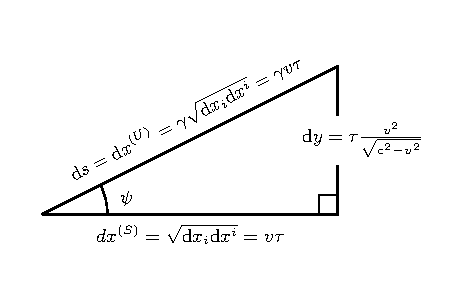
\includegraphics[width=0.75\textwidth]{../diagrams/outputs/simple_triangle.eps}
\caption{A path element through $\mathbb{R}^3\times y$: the advance $dx$ through $\mathbb{R}^3$, the advance $dy$ along the density axis, and the path length $ds=dx^{(U)}=\gamma\,dx$. The inclination $\psi$ of the path satisfies $\tan\psi=\partial_x y=\beta\gamma$ (subsection~\ref{sec_paths}).}
\label{fig_trig_diagram}
\end{figure}

\subsection{The Lighthouse \& The Clock-Tower}\label{sec_lighthouse}

The picture can be stated as a thought experiment. Let $\mathbf{S}$ be the absolute frame, and let two observers, $A$ and $B$, agree that $B$ will travel at an agreed speed $v$ relative to $\mathbf{S}$ between two points $p_1$ and $p_2$ at rest in $\mathbf{S}$, a distance $d$ apart. $A$ remains at $p_1$. At $p_2$ stands a clock tower large enough to be read from $p_1$. Its face is read by the light it sends out: a lighthouse, whose light spreads from each event as a sphere of radius $c\,\Delta t$.

We make two assertions.

\begin{enumerate}[label=\arabic*.]
\item To keep a classical simultaneity in $\mathbb{R}^{3}$, $A$ and $B$ must agree on the time at which $B$ reaches $p_{2}$.
\item To agree with the measured dilation of moving clocks~\cite{Rossi1941, FrischSmith1963, Bailey1977, Bailey1979, Botermann2014}, the clock carried by $B$ must advance by $d/(\gamma v)$ on the trip.
\end{enumerate}

Both hold if the motion of $B$ is a path through $\mathbb{R}^3\times y$ (subsection~\ref{sec_paths}). Along it $B$ advances $d$ through $\mathbb{R}^3$ and $\beta\gamma d$ along $y$, so the path has length $\gamma d$. The absolute time of the trip,

\begin{equation}\label{eq_lighthouse_time}
    \Delta\tau=\frac{d}{v}=\frac{\gamma d}{\gamma v},
\end{equation}

is the same whether it is formed from the absolute distance and speed, as $A$ does, or from the path length and the rate $\gamma v$ along the path, as $B$ does. In the second form the speed is divided by the coordinate density $1/\gamma$: a speed referred to the path dilates inversely with the coordinate density. The clock of $B$ reads $d/(\gamma v)$ (subsection~\ref{sec_paths}), which satisfies the second assertion. The light from the clock tower does not define the time of the trip; it is how the time is read. Because every reading is carried by light, time appears to pass at $c$. A photon is the limit of the construction in which the path turns entirely along $y$ and the coordinate density vanishes (subsection~\ref{sec_paths}).

\section{Motion without Time}\label{sec_motion}

This section builds the kinematics of SR from the two properties of time that the model keeps: a fourth displacement coordinate, the position along $y$, and a driving rate of change, motion. Throughout, $\mathbf{S}$ is the absolute frame in which $\mathbb{R}^3$ is at rest, and $\tau$ is its time. $\tau$ is not an independent coordinate: subsection~\ref{sec_paths} obtains $c\tau$ as a ratio of lengths along a path, so seconds enter only through the value of $c$. We also require that, in a frame co-moving along $y$, mechanical equations reduce to their Newtonian forms, with only the relativistic part of each magnitude extending along $y$. Table~\ref{table_dictionary} lists the quantities used and their standard counterparts.

\begin{table}[h]
\caption{Quantities of this paper and their standard counterparts}%
\label{table_dictionary}
\begin{tabular}{@{}p{0.40\linewidth}p{0.54\linewidth}@{}}
\toprule
This paper & Standard counterpart\\
\midrule
$\psi$, $\tan\psi=\partial_x y$ & inclination of a path, or of space around a mass, in $\mathbb{R}^3\times y$; $\psi=\mathrm{gd}(\eta)$, the Gudermannian of the rapidity\\
$\sin\psi=\beta=v/c$ & speed; in gravity the flow velocity, which is the shift vector (``river velocity'') and the escape velocity from the enclosed mass\\
$\cos\psi=1/\gamma$ & coordinate density; the rate of a moving clock, and of a static clock outside a mass (co-expansion)\\
$c\,d\tau=dx\,ds/dy$, $c\,dt_U=dx^2/dy$ & absolute time and proper time of a moving clock\\
$y(r)$, $\partial_r y=\beta\gamma$ & inclination of space around a mass; $r$ is the absolute radius\\
$R=\gamma r$ & measured (areal) radius of a co-expanded sphere\\
$\partial_\tau y=v^2/\sqrt{c^2-v^2}$ & $dy/dT$ along a worldline at rest in the outward flow\\
\bottomrule
\end{tabular}
\end{table}

\subsection{The Fourth Coordinate and the Lorentz Factor}\label{sec_fourth_coordinate}

Let a body move at speed $v$ relative to $\mathbf{S}$, and let the additional coordinate grow along its motion as

\begin{equation}\label{eq_dy_definition}
    y=\tau\frac{v^2}{\sqrt{c^2-v^2}} .
\end{equation}

With $x=v\tau$ this gives

\begin{equation}\label{eq_dy_dtau}
    \partial_\tau y=\frac{v^2}{\sqrt{c^2-v^2}}=\frac{\gamma v^2}{c},
\end{equation}

\begin{equation}\label{eq_dy_dx}
    \partial_x y=\frac{v}{\sqrt{c^2-v^2}}=\beta\gamma ,
\end{equation}

and $v\,\partial_x y=\partial_\tau y$. Squaring equation~\eqref{eq_dy_dx} and using $\gamma^2=1/(1-\beta^2)$ gives

\begin{equation}\label{eq_gamma_dy_dx}
    \gamma=\sqrt{1+\left(\partial_x y\right)^2},
\end{equation}

so the Lorentz factor is the slope of the additional coordinate. The length of a path element through $\mathbb{R}^3\times y$ is then

\begin{equation}\label{eq_path_length}
    ds^2=dx^2+dy^2=\gamma^2dx^2 .
\end{equation}

This is the separation $dx'=\gamma\,dx$ that the Lorentz transformation assigns, in the frame $\mathbf{U}$ moving at $v$, to two events separated by $dx$ at equal $\tau$. The same transformation gives $c\,dt'=-\gamma(v/c)\,dx=-dy$ for these events, and the interval is preserved, $c^2dt'^2-dx'^2=dy^2-\gamma^2dx^2=-dx^2$. Subsection~\ref{sec_classical_simultaneity} extends this from equal-$\tau$ separations to arbitrary events. The relation to the rapidity $\eta$ is elementary: $\gamma=\cosh\eta$ and $\partial_x y=\sinh\eta$, so equation~\eqref{eq_gamma_dy_dx} is the identity $\cosh^2\eta=1+\sinh^2\eta$.

\subsection{Motion as Paths through \texorpdfstring{$\mathbb{R}^3\times y$}{R3 x y}}\label{sec_paths}

A motion is a path through $\mathbb{R}^3\times y$. It carries no time parameter; its only property at each point is its direction. Let $\psi$ be the inclination of the path above $\mathbb{R}^3$ (figure~\ref{fig_trig_diagram}). Equation~\eqref{eq_dy_dx} gives $\tan\psi=\partial_x y=\beta\gamma$, and hence

\begin{equation}\label{eq_path_angle}
    \sin\psi=\frac{dy}{ds}=\beta,
    \qquad
    \cos\psi=\frac{dx}{ds}=\frac{1}{\gamma}.
\end{equation}

The two direction cosines are the rates of the model. The speed is the advance along $y$ per unit path, $\sin\psi$: a body is propelled along the density axis by its motion, and its speed is that propulsion. The fraction $\cos\psi$ of the path that lies in $\mathbb{R}^3$ is the coordinate density, the number of absolute coordinates per measured length, and it is also the rate of a clock carried along the path.

\paragraph{Time readings as ratios of distances.} Along a path element with advances $dx$ and $dy$, the absolute time and the reading of a clock carried along the path are

\begin{equation}\label{eq_path_times}
    c\,d\tau=\frac{dx\,ds}{dy}=\frac{dx}{\sin\psi},
    \qquad
    c\,dt_U=\frac{dx^2}{dy}=\frac{dx}{\tan\psi}.
\end{equation}

They give $dx=v\,d\tau$, the moving-clock rate $dt_U=d\tau/\gamma$, and $c\,dt_U=\gamma c\,d\tau-dy$ along the path, which are items 4 and 1 of the Proposition in subsection~\ref{sec_classical_simultaneity}. Neither reading is an independent coordinate. Both are lengths formed from the path.

\paragraph{The causal sphere.} Light spreads from each event as a sphere of radius $c\,d\tau$. While a body advances $dx$ through $\mathbb{R}^3$ the sphere reaches $c\,d\tau=dx/\sin\psi$, so

\begin{equation}\label{eq_causal_sphere}
    \frac{dx}{c\,d\tau}=\sin\psi\leq1 ,
\end{equation}

and every body remains inside the causal sphere of its own past events. This is the only place where $c$ enters. The path itself does not advance at $c$: its length per unit of light distance, $ds/(c\,d\tau)=\beta\gamma=\tan\psi$, takes any value. Time is read off the causal sphere, so it appears to pass at $c$; the rate of change that the model identifies with time is the motion along the four axes, which is not bound to that rate. Whether the two rates can be told apart by measurement is discussed in subsection~\ref{sec_two_rates}.

\paragraph{Composition.} With $\tanh\eta=\beta$, the inclination is the Gudermannian of the rapidity, $\psi=\mathrm{gd}(\eta)=\arctan(\sinh\eta)$. Collinear motions compose by adding rapidities, so $\sin\psi_W=\tanh(\eta_1+\eta_2)=(\beta_1+\beta_2)/(1+\beta_1\beta_2)$, the relativistic composition of velocities.

\paragraph{Limits.} A body at rest has no path ($dx=dy=0$), and equation~\eqref{eq_path_times} gives it no time reading of its own. Its time must come from other change: its internal motion, or the motion of everything else, as in ephemeris time~\cite{Barbour2009}. Light is the limit $\psi\to90^\circ$, in which the coordinate density $\cos\psi$ vanishes, the clock reading $c\,dt_U$ goes to zero, and $c\,d\tau$ goes to $dx$, the radius of the causal sphere. The limit is consistent but degenerate.

\paragraph{Relation to Euclidean relativity.} Euclidean relativity~\cite{Montanus2001,Almeida2001} writes $(c\,d\tau)^2=dx^2+(c\,d\tau_p)^2$, with the proper time $\tau_p$ as a fourth spatial coordinate, and postulates that everything moves through that space at $c$. Its worldline makes the angle $\psi$ with the proper-time axis, $\tan\psi=dx/(c\,d\tau_p)=\beta\gamma$. The path triangle $(dx,dy;ds)$ of this paper is therefore similar to its triangle $(c\,d\tau_p,dx;c\,d\tau)$, scaled by $\tan\psi$. The postulate is not used here, and the constructions differ: the path of this paper advances at $ds/(c\,d\tau)=\tan\psi$, not at $c$.

The next subsection uses these readings to show that every inertial observer recovers the same absolute time.

\subsection{Classical Simultaneity in \texorpdfstring{$\mathbb{R}^3$}{R3}}\label{sec_classical_simultaneity}

Subsection~\ref{sec_fourth_coordinate} treated two events at equal $\tau$. Here, once the displacement along $y$ is included, every inertial observer assigns the same absolute time $\tau$ to every event, and the relativity of simultaneity is entirely a displacement along $y$.

Let events be labelled by an absolute position $x$ in $\mathbb{R}^3$ (one axis is shown) and by the absolute time $\tau$, both referred to the frame $\mathbf{S}$. An observer $\mathbf{U}$ moving at velocity $v$ relative to $\mathbf{S}$ assigns to each event the displacement

\begin{equation}\label{eq_y_offset}
    y_U(x)=\gamma\frac{v}{c}\,x ,
\end{equation}

which is equation~\eqref{eq_dy_dx} integrated at fixed velocity.

\paragraph{Proposition.} For every event $(x,\tau)$ and every inertial observer $\mathbf{U}$ moving at $v$ relative to $\mathbf{S}$:
\begin{enumerate}
\item the Lorentz coordinates of $\mathbf{U}$ are
\begin{equation}\label{eq_observer_clock}
    x_U=\gamma\left(x-v\tau\right),
    \qquad
    c\,t_U=\gamma c\,\tau-y_U(x) ;
\end{equation}
\item every observer recovers the same absolute time,
\begin{equation}\label{eq_tau_recovered}
    \tau=\frac{c\,t_U+y_U(x)}{\gamma c} ;
\end{equation}
\item two events with $\Delta\tau=0$ and any separation $\Delta x$ satisfy $c\,\Delta t_U=-\Delta y_U$;
\item along the worldline of $\mathbf{U}$, $x=v\tau$, the clock of $\mathbf{U}$ advances by $dt_U=d\tau/\gamma$;
\item for an observer $\mathbf{W}$ moving at $v_2$ relative to $\mathbf{U}$, items 1 to 4 hold with $v$ replaced by the velocity of $\mathbf{W}$ relative to $\mathbf{S}$, $v_W=(v+v_2)/(1+vv_2/c^2)$.
\end{enumerate}

\begin{proof}
1. With $\tau$ as the time coordinate of $\mathbf{S}$, the Lorentz transformation gives $x_U=\gamma(x-v\tau)$ and
\begin{equation}
    c\,t_U=\gamma\left(c\tau-\frac{v}{c}x\right)=\gamma c\,\tau-\gamma\frac{v}{c}x=\gamma c\,\tau-y_U(x),
\end{equation}
using equation~\eqref{eq_y_offset}.

2. Solving equation~\eqref{eq_observer_clock} for $\tau$ gives equation~\eqref{eq_tau_recovered}. The right-hand side uses only quantities assigned by $\mathbf{U}$ and its velocity relative to $\mathbf{S}$, and it returns the same $\tau$ for every $v$.

3. Subtracting equation~\eqref{eq_observer_clock} for two events at equal $\tau$ gives $c\,\Delta t_U=-\gamma(v/c)\Delta x=-\Delta y_U$.

4. On $x=v\tau$, $y_U=\gamma v^2\tau/c$, so
\begin{equation}
    c\,t_U=\gamma c\,\tau\left(1-\frac{v^2}{c^2}\right)=\frac{c\,\tau}{\gamma}.
\end{equation}
The clock of $\mathbf{U}$ loses, relative to $\gamma c\,d\tau$, exactly its own advance $dy_U=\gamma(v/c)\,v\,d\tau$ along $y$.

5. Collinear boosts compose by addition of rapidities, so the boost at $v$ followed by the boost at $v_2$ is the boost at $v_W$ with $\gamma_W=\gamma\gamma_2(1+vv_2/c^2)$. Items 1 to 4 then follow with $v_W$ and $y_W(x)=\gamma_W(v_W/c)\,x$.
\end{proof}

The conventional time difference $\Delta t_U=-\gamma v\Delta x/c^2$ between two events at the same $\tau$ is therefore not a difference in absolute time. It is the displacement $\Delta y_U$ that $\mathbf{U}$ assigns to their separation, and all of $\mathbb{R}^3$ at a given $\tau$ is one instant for every observer. Item 4 obtains the slowing of a moving clock from its displacement along $y$; it does not insert time dilation separately. In the language of subsection~\ref{sec_paths}, the clock rate $1/\gamma$ is the coordinate density $\cos\psi$ of the path. For $\Delta\tau=0$ the absolute separation is the same for every observer, $\Delta x^2=\Delta x_U^2-(c\Delta t_U)^2=\Delta x_U^2-\Delta y_U^2$. This is the embedding relation $\Delta x_U^2=\Delta x^2+\Delta y_U^2$ read with the absolute length as the invariant. The separation $\Delta x_U$ measured by $\mathbf{U}$ is the hypotenuse of the graph of $y_U$ over $\mathbb{R}^3$ and depends on the observer, while its projection $\Delta x$ onto $\mathbb{R}^3$ does not. With $w=c\tau$, a length, item~1 reads $x_U=\gamma\left(x-\beta w\right)$ and $w_U=c\,t_U=\gamma w-y_U$. The transformation acts on lengths alone, and its invariant, $x_U^2-w_U^2=x^2-w^2$, is the Minkowski interval written in them; the geometry of subsection~\ref{sec_paths} reads the same transformation as the inclination of a path.

The frame $\mathbf{S}$ is an assumption of the model. Nothing in the kinematics singles it out, and every local experiment gives the same result in it as in any other inertial frame. We identify it with the frame of the flow of space: the cosmic rest frame on large scales, whose velocity relative to an observer is measured by the dipole of the cosmic microwave background, and the outward flow of section~\ref{sec_gravity} near a mass. The next section shows that the same inclination, and the same offset along $y$, appear in gravity once matter co-expands with $y$.

\section{Co-expansion and Gravity}\label{sec_gravity}

In SR the inclination of a path is set by the speed of the body. In gravity it is set by the flow of space, and the geometry needs one further ingredient, which is how matter responds to the inclination. This section states that response as a postulate, shows that it gives the equivalence principle, and derives the geometry of space around a mass from it.

\subsection{Co-expansion}\label{sec_coexp_postulate}

In SR a moving observer assigns the length $ds=\gamma\,dx$ to an absolute separation $dx$ along its motion (equation~\eqref{eq_path_length}), and its clock runs at $1/\gamma$. The same factor governs bodies at rest near a mass, in every direction:

\paragraph{Postulate (co-expansion).} All matter co-expands with the change in $y$. Every material length, of a ruler, an atom or the Earth, is scaled by the local Lorentz factor $\gamma$ of the inclination of space into $y$, and every clock runs at the coordinate density $1/\gamma$.

Measured with co-expanding rulers and clocks, an interval with absolute separation $d\mathbf{x}$ and static time $dt$ has
\begin{equation}\label{eq_coexp_static}
    ds^2=-\frac{c^2dt^2}{\gamma^2}+\gamma^2\,|d\mathbf{x}|^2 .
\end{equation}
The scaling is the same for every kind of matter. The motion of a body in equation~\eqref{eq_coexp_static} therefore cannot depend on what the body is made of, and the universality of free fall is a property of the geometry rather than a separate principle. Co-expansion is in this sense the origin of the equivalence principle. It is not observable locally: every ruler and every clock at a point co-expands by the same factor, so a local measurement compares only co-expanded quantities with one another.

\subsection{The Outward Flow}\label{sec_pg_relation}

Let $T$ be the absolute time, the proper time of observers at rest in absolute space, and let $r$ be the absolute radius from a mass $M$. Space flows radially outward from the mass, in the same direction as the Hubble flow, at the speed $\beta c$ relative to an observer held at fixed $r$. In the absolute frame the line element is
\begin{equation}\label{eq_pg_metric}
    ds^2=-c^2dT^2+\left(dr-\beta c\,dT\right)^2+\gamma^2r^2d\Omega^2,
    \qquad
    \gamma=\frac{1}{\sqrt{1-\beta^2}} .
\end{equation}
It has unit lapse, so $T$ is the proper time of the observers at rest in absolute space, and their worldlines are geodesics. The angular part carries the co-expansion: a sphere of absolute radius $r$ has the measured circumference $2\pi\gamma r$. Section~\ref{sec_inclined_space} shows that equation~\eqref{eq_pg_metric} is equation~\eqref{eq_coexp_static} written in the absolute frame. Removing the angular co-expansion, $\gamma^2r^2\to r^2$, gives the Painlev\'e--Gullstrand form of the Schwarzschild metric~\cite{Painleve1921,Gullstrand1922,MartelPoisson2001}, with its flow reversed to point outward. The inward form is the river model~\cite{HamiltonLisle2008}. The outward direction is a postulate of the model.

\paragraph{The flow is set by the measured radius.} The flow speed is the escape velocity from the mass,
\begin{equation}\label{eq_flow_measured}
    \beta^2=\frac{2GM}{c^2R},
    \qquad
    R=\gamma r ,
\end{equation}
where $R$ is the measured radius of a co-expanded sphere, $2\pi R$ its measured circumference. The radius must be the measured one because the mass that sources the flow has itself co-expanded. With $u=GM/(c^2r)$, equation~\eqref{eq_flow_measured} reads $\beta^2=2u/\gamma$, and with $\beta^2=1-1/\gamma^2$ it fixes the Lorentz factor:
\begin{equation}\label{eq_gamma_selfconsistent}
    \gamma^2-2u\gamma-1=0,
    \qquad
    \gamma=u+\sqrt{1+u^2}.
\end{equation}
The measured radius of a sphere is then $R=GM/c^2+\sqrt{(GM/c^2)^2+r^2}$, which exceeds the absolute radius by $GM/c^2$ to leading order. At the surface of the Earth space streams outward at the escape velocity, about $11.2~\mathrm{km\,s^{-1}}$, and the Earth's measured radius exceeds its absolute radius by about $4.4$~mm. Neither is visible locally, because every ruler on the Earth co-expands with it.

If the flow were set instead by the absolute radius, $\beta^2=2u$, equation~\eqref{eq_coexp_static} would have the post-Newtonian parameters $\gamma_{\rm PPN}=1$ and $\beta_{\rm PPN}=0$. The perihelion advance would then be $(2+2\gamma_{\rm PPN}-\beta_{\rm PPN})/3=4/3$ of the general-relativistic value, which the orbit of Mercury excludes~\cite{Will2014}. Co-expansion therefore fixes not only the scaling of matter but also the radius that sets the flow. Subsection~\ref{sec_field_equation} shows that this rule is the point-mass solution of a linear field equation.

\paragraph{The Hubble flow.} For flat FLRW cosmology, $R=a(t)r$ gives the same outward form with $\beta_H=HR/c$, and the Hubble radius $c/H$, where $\beta_H=1$, is its apparent horizon~\cite{Faraoni2011,Faraoni2022}. With $m=\tfrac{4\pi}{3}\rho R^3$ and the Friedmann equation $H^2=8\pi G\rho/3$, the Hubble flow obeys $\beta_H^2=2Gm/(c^2R)$, the relation of equation~\eqref{eq_flow_measured} with the enclosed mass, and its Newtonian counterpart is the zero-energy condition of Milne and McCrea~\cite{Milne1934,McCreaMilne1934}. Binding and expansion are one outward flow with different distributions of mass. The Friedmann equation is imported from general relativity here, and the co-expansion form of an expanding universe is not developed in this paper.

\subsection{The Field Equation}\label{sec_field_equation}

Dividing equation~\eqref{eq_gamma_selfconsistent} by $\gamma$ gives $\gamma-1/\gamma=2GM/(c^2r)$. The right-hand side is $-2/c^2$ times the Newtonian potential of the mass in absolute coordinates, which is harmonic away from the mass. The self-consistent Lorentz factor is therefore the point-mass solution of a linear equation in flat absolute space,
\begin{equation}\label{eq_field_equation}
    \nabla^2\!\left(\gamma-\frac{1}{\gamma}\right)=-\frac{8\pi G}{c^2}\,\sigma ,
\end{equation}
where $\nabla^2$ is the Laplacian of absolute coordinates and $\sigma$ is the density that sources the field, found below. Outside matter $\sigma=0$. The equation is linear in the field $\psi\equiv\gamma-1/\gamma=\gamma\beta^2=-2\Phi/c^2$, not in $\gamma$, and its solution is
\begin{equation}\label{eq_gamma_asinh}
    \gamma=\exp\!\left[\operatorname{asinh}\!\left(-\frac{\Phi}{c^2}\right)\right],
\end{equation}
with $\Phi$ the Newtonian potential of $\sigma$ in absolute space; for a point mass this is $\gamma=u+\sqrt{1+u^2}$. The measured radius in equation~\eqref{eq_flow_measured} is therefore not a choice made to pass the perihelion test: it is what the field equation gives for a point mass. With $|\nabla y|=\beta\gamma=\sqrt{\gamma^2-1}$ the field is $\psi=|\nabla y|^2/\sqrt{1+|\nabla y|^2}$, and equation~\eqref{eq_field_equation} is an equation for the height of the inclined space,
\begin{equation}\label{eq_field_equation_y}
    \nabla^2\frac{|\nabla y|^2}{\sqrt{1+|\nabla y|^2}}=-\frac{8\pi G}{c^2}\,\sigma ,
\end{equation}
which in the weak field reduces to $|\nabla y|^2=-2\Phi/c^2$.

\paragraph{The source inside matter.} Bodies move along the co-expansion geometry: this is their co-motion along $y$, and it is what gives the equivalence principle. A field term whose vacuum solutions are harmonic in $\psi$ must be $|\nabla\psi|^2$, so the simplest action for the field and matter is
\begin{equation}\label{eq_action}
    S=-\frac{c^4}{32\pi G}\int|\nabla\psi|^2\,d^3x\,dt-\sum m c^2\int\sqrt{\frac{1}{\gamma^2}-\frac{\gamma^2v^2}{c^2}}\;dt .
\end{equation}
A body of rest mass $m$ at rest has energy $mc^2/\gamma$, and $d(1/\gamma)/d\psi=-1/(1+\gamma^2)$, so varying $\psi$ gives the source
\begin{equation}\label{eq_source_coexp}
    \sigma=\frac{2\rho}{1+\gamma^2},
\end{equation}
with $\rho$ the rest mass per absolute volume. The same factor governs the fall. A body that is not co-moving falls relative to co-moving matter, such as the surface of the Earth, with the acceleration
\begin{equation}\label{eq_fall}
    a=\frac{c^2}{\gamma^2}\left|\frac{d\gamma}{dr}\right|=\frac{2GM}{r^2(1+\gamma^2)}=\frac{GM}{R^2\left(1-GM/(c^2R)\right)},
\end{equation}
which is $GM/r^2$ in the weak field; the value for a static observer in general relativity, $GM/[R^2\sqrt{1-2GM/(c^2R)}]$, agrees at first order. A coupling chosen so that the source would be exactly $\rho$ requires a static clock rate $1-\psi/2$, which gives $\beta_{\rm PPN}=\tfrac12$ and a perihelion advance $7/6$ of the general-relativistic value; the orbit of Mercury excludes it. Section~\ref{sec_sep} shows that the same action gives equal gravitational and inertial masses for self-gravitating bodies at first order.

\paragraph{Several masses and interiors.} Outside matter $\psi$ obeys a linear equation, so the geometry of any set of point masses at rest is exact, $\gamma-1/\gamma=(2G/c^2)\sum_iM_i/|\mathbf{x}-\mathbf{x}_i|$, with $M_i$ the gravitational masses (subsection~\ref{sec_several_masses}). Inside a body the source depends on $\gamma$ itself. To leading order in the interior field, $\sigma\simeq\rho$, and for a ball of uniform density and absolute radius $a$, $\psi=(GM/c^2)(3a^2-r^2)/a^3$, with the central clock rate
\begin{equation}\label{eq_ball_center}
    \frac{1}{\gamma(0)}=\exp\!\left[-\operatorname{asinh}\!\left(\frac{3GM}{2c^2a}\right)\right],
\end{equation}
which is positive for every compactness. With this leading-order source an incompressible star in hydrostatic equilibrium has a finite central pressure at every compactness, and its measured surface radius, $GM/c^2+\sqrt{(GM/c^2)^2+a^2}$, always exceeds $2GM/c^2$: the endpoint of collapse would be a horizonless object whose surface approaches the absolute centre. These interior results are provisional until the full source of equation~\eqref{eq_source_coexp} is used, and realistic equations of state and the observational limits on surfaces around black-hole candidates remain to be examined.

\paragraph{Status.} The field equation, its point-mass solution and the source inside matter follow from the action~\eqref{eq_action}. Its extension to moving sources (section~\ref{sec_kk}) and the strong-field behaviour of self-gravitating bodies (section~\ref{sec_sep}) are open.

\subsection{The Inclined Space}\label{sec_inclined_space}

An observer held at fixed $r$ moves inward relative to space at $-\beta c$. Its rest space has the radial component
\begin{equation}\label{eq_rest_space}
    h_{rr}=g_{rr}-\frac{g_{Tr}^2}{g_{TT}}=1+\beta^2\gamma^2=\gamma^2 ,
\end{equation}
so it measures $d\ell=\gamma\,dr$ radially. This factor is the Lorentz factor of its motion through the flow, as in SR. Its angular measurements, $\gamma r\,d\Omega$, carry the same factor through co-expansion. The static observer therefore measures $\gamma|d\mathbf{x}|$ in every direction: the radial factor comes from its motion through space, the angular factor from the co-expansion of the space itself, and the two are equal.

The space around a mass is inclined into $y$ exactly as a path is (figure~\ref{fig_trig_diagram}), with the flow speed in place of the speed of a body:
\begin{equation}\label{eq_flamm_slope}
    \partial_r y=\beta\gamma,
    \qquad
    \sin\psi=\beta,
    \qquad
    \cos\psi=\frac{1}{\gamma}=\frac{dr}{d\ell}.
\end{equation}
The radial measured length is the arc length of the graph of $y$ over the absolute radius, $d\ell^2=dr^2+dy^2$. A graph alone would leave circumferences unchanged; co-expansion supplies the equal angular factor, so that the measured geometry is isotropic.

\paragraph{The height is the synchronization offset.} The change of time $dT=dt-\beta\gamma^2\,dr/c$ takes the flow form~\eqref{eq_pg_metric} to the static form
\begin{equation}\label{eq_static_form}
    ds^2=-\frac{c^2dt^2}{\gamma^2}+\gamma^2\left(dr^2+r^2d\Omega^2\right),
\end{equation}
which is equation~\eqref{eq_coexp_static}. The cross term vanishes because $(1-\beta^2)\beta\gamma^2=\beta$, and the radial coefficient is $1+\beta^2\gamma^2=\gamma^2$. The offset between the absolute time $T$ and the static time $t$ is
\begin{equation}\label{eq_sync_gap_flamm}
    c\left(dT-dt\right)=-\beta\gamma^2\,dr=-\gamma\left(\beta\gamma\,dr\right)=-\gamma\,dy .
\end{equation}
In the proper time of the static observer, $c\,(dT-dt)/\gamma=-dy$: the offset is the height itself. The static observer moves inward relative to space at $-\beta c$, so light it sends outward travels with the flow at $c(1+\beta)$ and returns against it at $c(1-\beta)$. Its synchronization parameter is $\epsilon=(1-\beta)/2$~\cite{Reichenbach1958}, the value $\tfrac12(1+u/c)$ of an observer moving at $u$, and $dy=(1-2\epsilon)\,d\ell$. The structure is that of item~3 of the Proposition: absolute space supplies the observer-independent base $dr$, the static proper length $\gamma\,dr$ is the arc length of the graph, and a separation along $y$ is a difference in clock setting at one absolute time.

\paragraph{Coordinate density.} Equation~\eqref{eq_static_form} gives
\begin{equation}\label{eq_density_lapse}
    \frac{|d\mathbf{x}|}{d\ell}=\frac{1}{\gamma}=\cos\psi=\frac{d\tau_{\rm static}}{dt}
\end{equation}
in every direction: the number of absolute coordinates per measured length equals the rate of a static clock. In vacuum the coordinate density and the rate of time are one quantity, as for a moving clock in SR (subsection~\ref{sec_paths}).

\subsection{The Exact Metric}\label{sec_exact_metric}

With the measured radius $R=\gamma r$ as coordinate, $r=\sqrt{R^2-2GMR/c^2}$, $\gamma=1/\sqrt{1-2GM/(c^2R)}$, and equation~\eqref{eq_static_form} becomes, with $G=c=1$,
\begin{equation}\label{eq_coexp_areal}
    ds^2=-\left(1-\frac{2M}{R}\right)dt^2+\frac{(R-M)^2}{(R-2M)^2}\,dR^2+R^2d\Omega^2 .
\end{equation}
Its clock rate and its areal radius are those of the Schwarzschild metric. Only the radial component differs, by
\begin{equation}\label{eq_grr_ratio}
    \frac{g_{RR}}{g_{RR}^{\rm Schw}}=1+\frac{M^2}{R(R-2M)} .
\end{equation}
In the isotropic coordinates of equation~\eqref{eq_static_form},
\begin{equation}\label{eq_ppn_expansion}
    \frac{1}{\gamma^2}=1-2u+2u^2-u^3+O(u^4),
    \qquad
    \gamma^2=1+2u+2u^2+O(u^3),
\end{equation}
so that $\gamma_{\rm PPN}=\beta_{\rm PPN}=1$. The isotropic Schwarzschild metric has $1-2u+2u^2-\tfrac32u^3$ and $1+2u+\tfrac32u^2$, so the two first differ at second post-Newtonian order.

\paragraph{The centre.} As $r\to0$, $R\to2M$: the surface $R=2M$, where the static clock rate vanishes, is the absolute centre, and there is no region inside it. Along a static slice it lies at infinite proper radial distance, since $\int(R-M)\,dR/(R-2M)$ diverges logarithmically. A body falling radially from rest at infinity nevertheless reaches it in finite proper time, because $\dot R^2\simeq2(R-2M)/M$ near $R=2M$. What happens to matter that arrives at the centre is not determined here.

\subsection{The Geometry in the Language of General Relativity}\label{sec_effective_source}

Equation~\eqref{eq_coexp_areal} is not a vacuum solution of the Einstein equations. Read through them, it is the field of a mass $M$ together with an exterior source. With $2m(R)=R\left(1-1/g_{RR}\right)$ and the static Einstein equations,
\begin{equation}\label{eq_effective_mass}
    m(R)=\frac{MR(2R-3M)}{2(R-M)^2},
\end{equation}
\begin{equation}\label{eq_effective_source}
    8\pi\rho_{\rm eff}=-\frac{M^2(R-3M)}{R^2(R-M)^3},
    \qquad
    8\pi p_r=-\frac{M^2}{R^2(R-M)^2},
    \qquad
    p_t=-p_r .
\end{equation}
Far from the mass, $\rho_{\rm eff}\simeq p_r\simeq-g^2/(8\pi G)$ with $g=GM/R^2$ (restoring $G$ and $c=1$). This is the energy density of the Newtonian gravitational field, which is negative. In the language of general relativity, co-expansion is the geometry in which the field's own energy acts as a source. The mass function returns to $m=M$ at infinity and at $R=2M$, and reaches its maximum, $9M/8$, at the photon sphere $R=3M$. Including the energy of the gravitational field as a source was the central idea of Yilmaz~\cite{Yilmaz1958}. Here it is not added to the field equations; it follows from a postulate about how matter responds to the inclination of space.

\subsection{Several Masses}\label{sec_several_masses}

By equation~\eqref{eq_field_equation} the field $\gamma-1/\gamma$ of several masses at rest is the sum of their single-mass fields, exactly; to first order
\begin{equation}
    \gamma^2=1+\frac{2G}{c^2}\sum_i\frac{M_i}{r_i}+O\!\left(u^2\right),
\end{equation}
and the measured geometry $\gamma^2|d\mathbf{x}|^2$ is conformally flat. This is the instantaneous geometry of masses at rest; how it changes as they move is the time-dependent problem. In general relativity separated masses at rest have no static vacuum solution without stresses to hold them apart, and the time-symmetric initial slice of several masses is conformally flat, with a conformal factor that superposes linearly~\cite{BrillLindquist1963}. If, instead, the measured geometry were the metric induced on a single hypersurface $y=h(\mathbf{x})$, as for the radial direction in equation~\eqref{eq_flamm_slope}, two masses could not be described: in the weak field the Gauss equation can be solved point by point for the second derivatives of $h$, but the result fails the Codazzi equations, so it is not the Hessian of any height $h$ (the accompanying code checks this numerically). Co-expansion removes this obstruction, because the measured geometry is set by $\gamma$ and not by the induced metric. In the weak field the condition $\gamma^2=1+|\nabla h|^2=1-2\Phi/c^2$ is the eikonal equation $|\nabla h|^2=-2\Phi/c^2$ for the height of the inclined space. Where the outward flows of two bodies meet head-on, $\nabla h$ changes direction across a surface; the jump is normal to that surface, carries no vorticity, and exerts no force.

\subsection{The Rate of Change of Coordinate Density}\label{sec_coordinate_density}

The two properties of time that the model keeps, a fourth displacement coordinate and a rate of change, have a counterpart in the flow: the coordinate density of equation~\eqref{eq_density_lapse}, and the rate at which the flow changes it. The flow $\vec v$ of absolute space changes the coordinate density at the rate $\theta=\nabla\cdot\vec v$, the fractional rate of change of a volume element carried by the flow. On the absolute slices of equation~\eqref{eq_pg_metric}, whose volume element is $\gamma^2r^2\,dr\,d\Omega$,
\begin{equation}\label{eq_theta_mass}
    \theta=\frac{1}{R^2}\frac{d}{dr}\left(R^2\beta c\right)=\frac{3\beta c}{2R}\,\frac{r}{\sqrt{r^2+(GM/c^2)^2}} .
\end{equation}
For the Hubble flow, $\vec v=H\vec R$, $\theta=3H$, and the constraint and Raychaudhuri equations of general relativity~\cite{Raychaudhuri1955}, written for the flow, are the Friedmann and acceleration equations. Around a mass, the corresponding statement in the absolute slices of co-expansion requires the time-dependent field equations of the model, which are not yet known.
\section{Paths without Time}\label{sec_time_elimination}

Subsection~\ref{sec_paths} removed time from SR. For a steady flow the same can be done in gravity: the time coordinate can be eliminated exactly, leaving the paths of light and of bodies through absolute $\mathbb{R}^3$, with time readings derived from the paths afterwards. Here ``steady'' means that the flow does not change along itself, so that the geometry is stationary. It is not an assumption that time is periodic or compact: no coordinate is wrapped.

\paragraph{Light: the causal sphere carried by the flow.} In the absolute frame, equation~\eqref{eq_pg_metric}, light obeys $|d\mathbf{x}-\mathbf{W}\,dT|_h=c\,dT$, where $h$ is the metric $dr^2+\gamma^2r^2d\Omega^2$ of the absolute slice and $\mathbf{W}=\beta c\,\partial_r$ is the wind. The causal sphere spreads at $c$ relative to the outward-flowing space while being carried by it. This is Zermelo's navigation problem, and its travel time is the length of a Randers--Finsler metric~\cite{GibbonsZermelo2009}. For $W<c$,
\begin{equation}\label{eq_zermelo_time}
    dT=\frac{-\langle\mathbf{W},d\mathbf{x}\rangle_h+\sqrt{\langle\mathbf{W},d\mathbf{x}\rangle_h^2+\left(c^2-W^2\right)|d\mathbf{x}|_h^2}}{c^2-W^2}.
\end{equation}
Radially it gives $dr/dT=c(1+\beta)$ outward and $c(1-\beta)$ inward, as in subsection~\ref{sec_inclined_space}. In the static form, equation~\eqref{eq_static_form}, light obeys Fermat's principle with the optical metric $\gamma^4|d\mathbf{x}|^2$:
\begin{equation}\label{eq_optical_index}
    c\,dt=n\,|d\mathbf{x}|,
    \qquad
    n=\gamma^2 .
\end{equation}
Light therefore moves through flat absolute space as through a medium of refractive index $\gamma^2$, one factor of $\gamma$ from the co-expansion of lengths and one from the slowing of clocks. The two travel times differ by an exact differential,
\begin{equation}\label{eq_randers_fermat}
    c\,dT=c\,dt-\beta\gamma^2\,dr=c\,dt-\gamma\,dy ,
\end{equation}
which is the synchronization offset of equation~\eqref{eq_sync_gap_flamm}. An exact differential does not change the paths that extremize the travel time, so the two descriptions give the same light paths, and the height of the inclined space is the bridge between them.

\paragraph{Bodies with $v\neq c$.} A body does not move with the causal sphere, and its paths are not those of light. In a static field its paths at fixed energy $E$ per unit rest energy are the geodesics of the Jacobi metric~\cite{Gibbons2016Jacobi}, which for equation~\eqref{eq_static_form} is conformally flat:
\begin{equation}\label{eq_jacobi}
    J_{ij}=\left(E^2\gamma^2-1\right)\gamma^2\,\delta_{ij}.
\end{equation}
It is a positive-definite metric on absolute $\mathbb{R}^3$ with no time coordinate, and time is recovered afterwards along the path. Bodies, like light, move through flat space with an index of refraction, $\gamma\sqrt{E^2\gamma^2-1}$. In the absolute frame the corresponding metric is of Randers type~\cite{Chanda2019Jacobi}, and the reduced momenta in the two frames differ by $E$ times the same exact differential, so bodies also follow the same paths in both.

\paragraph{Orbits.} In the measured radius, with $u=1/R$, angular momentum $L$ per unit mass and $G=c=1$, the equatorial geodesics of equation~\eqref{eq_jacobi} give (appendix~\ref{app_orbits})
\begin{equation}\label{eq_jacobi_orbit}
    \left(\frac{du}{d\phi}\right)^2=\frac{(1-2Mu)\left[E^2-(1-2Mu)\left(1+L^2u^2\right)\right]}{L^2\left(1-Mu\right)^2}.
\end{equation}
Through first order in $M$ this is the Schwarzschild orbit equation,
\begin{equation}
    \left(\frac{du}{d\phi}\right)^2=\frac{E^2-1}{L^2}+\frac{2M}{L^2}u-u^2+2Mu^3+M^2\left(u^4+\frac{u^2}{L^2}-\frac{E^2u^2}{L^2}\right)+O(M^3),
\end{equation}
so the perihelion advance is $\Delta\phi=6\pi GM/[a(1-e^2)c^2]$ to leading order. Circular orbits, the innermost stable circular orbit and the photon sphere depend only on $g_{tt}$ and the areal radius, and are those of the Schwarzschild exterior: circular orbits have $L^2=MR^2/(R-3M)$, the innermost stable one is at $R=6M$, and light circles at $R=3M$ with critical impact parameter $b_c=3\sqrt3M$. For light,
\begin{equation}\label{eq_light_orbit}
    \left(\frac{du}{d\phi}\right)^2=\frac{(1-2Mu)\left(1/b^2-u^2+2Mu^3\right)}{(1-Mu)^2},
\end{equation}
and the deflection of a ray with impact parameter $b$ is
\begin{equation}\label{eq_deflection}
    \alpha=\frac{4M}{b}+4\pi\frac{M^2}{b^2}+O\!\left(\frac{M^3}{b^3}\right),
\end{equation}
compared with $4M/b+\tfrac{15\pi}{4}M^2/b^2$ in general relativity.

\paragraph{Scope.} The elimination is exact for the steady flow around an isolated mass. An expanding universe with varying $H$ is navigation in a wind that changes along the flow, and its time is not reduced to a fixed metric here. What the elimination shows is that, around a mass, nothing in the motion of light or of bodies requires a time dimension: the paths lie in flat absolute $\mathbb{R}^3$ with an index of refraction set by $\gamma$, the causal sphere supplies $c$, and time is read from the paths.

The density axis has so far been a flat fourth axis. Section~\ref{sec_kk} asks how it fits a five-dimensional metric, which is where a dynamics of its own would have to come from.
\section{The Unwrapped Kaluza--Klein Metric}\label{sec_kk}

Sections~\ref{sec_motion} to~\ref{sec_time_elimination} used $y$ as a fourth spatial axis with a flat metric. This section places it in a five-dimensional metric. The off-diagonal components then contain the potential generated by $y$ and the gravitomagnetic field of rotating sources, and the diagonal component gives a scalar sector.

\subsection{The Five-Dimensional Metric}

We represent the additional coordinate through the metric component $G_{44}$ of a five-dimensional metric,
\begin{equation}\label{eq_kk_line_element}
    dS^2=g_{\mu\nu}dx^\mu dx^\nu+G_{44}\,dy^2,
    \qquad
    G_{AB}=\begin{pmatrix} g_{\mu\nu} & 0\\ 0 & G_{44}\end{pmatrix}.
\end{equation}
The coordinate $y$ is not compactified. For a path, $dx^2+G_{44}\,dy^2$ with $dy=\beta\gamma\,dx$ reproduces $ds^2=\gamma^2dx^2$ only for $G_{44}=1$. In gravity the radial measured length of equation~\eqref{eq_flamm_slope}, $d\ell^2=dr^2+G_{44}\,dy^2$ with $\partial_ry=\beta\gamma$, requires the same normalization, $G_{44}=1$, to all orders. The angular co-expansion is not an embedding effect: it is the postulate of subsection~\ref{sec_coexp_postulate}, and it does not involve $G_{44}$.

\paragraph{Four-dimensional gravity from a non-compact dimension.} A flat, non-compact extra dimension does not by itself give four-dimensional gravity: if the field equations were obtained from a five-dimensional action integrated over $y$, the effective Newton constant would diverge. Induced-matter theory~\cite{Wesson1999STM,OverduinWesson1997} works instead with the five-dimensional field equations under the cylinder condition $\partial_y g_{\mu\nu}=\partial_y G_{44}=0$, and brane localization~\cite{RandallSundrum1999} is another route. A five-dimensional action for the model remains open.

\subsection{The Four-Potential and Rotation}\label{sec_four_potential}

In Kaluza--Klein geometry the off-diagonal components of the metric are the four-potential. Restoring them,
\begin{equation}\label{eq_kk_full}
    dS^2=g_{\mu\nu}\,dx^\mu dx^\nu+G_{44}\left(dy+\mathcal{A}_\mu dx^\mu\right)^2 .
\end{equation}
The line element is invariant under $y\to y+\Lambda(x)$, $\mathcal{A}_\mu\to\mathcal{A}_\mu-\partial_\mu\Lambda$. The density axis supplies a natural potential, evaluated in the rest frame of the source,
\begin{equation}\label{eq_potential_definition}
    \mathcal{A}_\mu\equiv\partial_\mu y,
    \qquad
    \mathcal{A}_0=0,
    \qquad
    \mathcal{A}_i=\beta\gamma\,\hat{n}_i ,
\end{equation}
and three identities follow:
\begin{align}
    \gamma^2 &= 1+\mathcal{A}_i\mathcal{A}^i,
    \label{eq_gamma_from_potential}\\
    \eta^{\mu\nu}\mathcal{A}_\mu\mathcal{A}_\nu &= \beta^2\gamma^2=\gamma^2-1,
    \qquad
    \mathcal{A}_\mu w^\mu=0,
    \label{eq_potential_norm}\\
    \mathcal{F}_{\mu\nu} &= \partial_\mu\mathcal{A}_\nu-\partial_\nu\mathcal{A}_\mu=0,
    \label{eq_potential_field_strength}
\end{align}
where $w^\mu$ is the four-velocity of an observer at rest relative to the source. The first is equation~\eqref{eq_gamma_dy_dx}; the second says that the potential is a spacelike covector orthogonal to $w^\mu$; the third holds because $\mathcal{A}_\mu$ is a gradient. The co-expansion factor of an isolated mass is therefore the pure-gauge sector, $\mathcal{F}_{\mu\nu}=0$, of the five-dimensional metric. The general potential is $\mathcal{A}_\mu=\partial_\mu y+a_\mu$, with field strength $\mathcal{F}_{\mu\nu}=\partial_\mu a_\nu-\partial_\nu a_\mu$, and a non-zero $a_\mu$ is the only way for the five-dimensional geometry to carry a field strength.

\paragraph{Rotation.} For a slowly rotating source, $a_\mu$ is the gravitomagnetic field. The gravitomagnetic field is a first post-Newtonian effect, the order at which co-expansion agrees with general relativity for static sources, and here we adopt the general-relativistic result at first order in the angular momentum $J$~\cite{Hartle1967}: space is dragged around the source at the angular velocity $\omega=2GJ/(c^2R^3)$~\cite{LenseThirring1918}. The azimuthal flow $\mathbf{v}_s=\omega\,\hat{\mathbf{z}}\times\mathbf{x}$ is the non-gradient component,
\begin{equation}\label{eq_nongradient_flow}
    a_i\simeq\frac{v_{s,i}}{c},
    \qquad
    \mathcal{F}=\nabla\times\mathbf{a}=\frac{2GJ}{c^3}\,\frac{3(\hat{\mathbf{z}}\cdot\hat{\mathbf{r}})\hat{\mathbf{r}}-\hat{\mathbf{z}}}{R^3},
\end{equation}
the vorticity of the flow, which has the form of a dipole field and is the gravitomagnetic field of the membrane paradigm~\cite{ThorneMembrane1986}. A gyroscope at rest precesses at $\boldsymbol{\Omega}_{\rm LT}=G\left[3(\mathbf{J}\cdot\hat{\mathbf{r}})\hat{\mathbf{r}}-\mathbf{J}\right]/(c^2R^3)$. Averaged over a polar orbit of radius $a$ this is $GJ/(2c^2a^3)$; for the Earth, $J_\oplus=5.86\times10^{33}~\mathrm{kg\,m^2\,s^{-1}}$ and $a=7027$~km, about $41~\mathrm{mas\,yr^{-1}}$, consistent within the accuracy of these rounded inputs with the Gravity Probe B measurement of $37.2\pm7.2~\mathrm{mas\,yr^{-1}}$~\cite{Everitt2011GPB}. Deriving rotation from co-expansion itself, rather than adopting it, is open.

\subsection{The Scalar Sector}

With $G_{44}=\Phi^2$, the cylinder condition and $c=1$, the five-dimensional Einstein equations $G^{(5)}_{AB}=\kappa_5T^{(5)}_{AB}$ reduce in the standard way~\cite{OverduinWesson1997} to
\begin{equation}\label{eq_effective_4d_field}
    G^{(4)}_{\mu\nu}=\kappa_5T^{(5)}_{\mu\nu}+\frac{1}{\Phi}\left(\nabla_\mu\nabla_\nu\Phi-g_{\mu\nu}\Box\Phi\right),
    \qquad
    \Box\Phi=-\frac{\kappa_5\Phi}{3}\left(\epsilon-3p+2p_y\right),
\end{equation}
for a perfect fluid with energy density $\epsilon$, pressure $p$ and stress $p_y$ along $y$. This is Brans--Dicke theory~\cite{BransDicke1961} with $\omega_{\rm BD}=0$. Outside a body the scalar obeys $\Box\Phi=0$. A sourced scalar with $\omega_{\rm BD}=0$ gives $\gamma_{\rm PPN}=\tfrac12$, excluded by the Cassini value $\gamma_{\rm PPN}-1=(2.1\pm2.3)\times10^{-5}$~\cite{Bertotti2003}, so $\Phi$ must be constant outside the body to that accuracy. The scalar is switched off only for the stress $p_y=(3p-\epsilon)/2$, which is a fine-tuning condition rather than a result. With $\Phi$ constant, equation~\eqref{eq_effective_4d_field} returns the Schwarzschild exterior. The second-order departure of co-expansion, equation~\eqref{eq_effective_source}, therefore cannot come from the scalar sector of the cylinder-condition reduction. In the static case the model supplies its own field equation, equation~\eqref{eq_field_equation}. Its extension to moving sources is the main open problem of the construction. A wave equation for the single field $\psi$ would be a scalar theory of gravity, which does not reproduce the orbital decay of binary pulsars or the tensor polarization of observed gravitational waves, so the time-dependent theory needs a tensor sector whose static limit is equation~\eqref{eq_field_equation}. Read through the Einstein equations, the exterior source of subsection~\ref{sec_effective_source} has $\rho\simeq p_r\simeq-p_t$ at leading order, the stress of a scalar field with negative kinetic energy, which suggests where to look.
\section{Where the Geometry Agrees with General Relativity and Where It Differs}\label{sec_gamma_coscaling}

\subsection{Gravity}

Table~\ref{table_coexp} compares the static geometry of an isolated mass with the Schwarzschild exterior.

\begin{table}[h]
\caption{The co-expansion geometry of an isolated mass compared with general relativity ($G=c=1$)}
\label{table_coexp}
\begin{tabular}{@{}p{0.36\linewidth}p{0.27\linewidth}p{0.29\linewidth}@{}}
\toprule
Quantity & Co-expansion & General relativity\\
\midrule
PPN $\gamma$, $\beta$ & $1$, $1$ & $1$, $1$\\
Static clock rate $g_{tt}$ (areal $R$) & $-(1-2M/R)$ & $-(1-2M/R)$\\
$g_{RR}$ & $(R-M)^2/(R-2M)^2$ & $1/(1-2M/R)$\\
$1/\gamma^2$ (isotropic $u$) & $1-2u+2u^2-u^3$ & $1-2u+2u^2-\tfrac32u^3$\\
Photon sphere, shadow $b_c$ & $3M$, $3\sqrt3M$ & $3M$, $3\sqrt3M$\\
Innermost stable orbit & $6M$ & $6M$\\
Light deflection & $4M/b+4\pi(M/b)^2$ & $4M/b+\tfrac{15\pi}{4}(M/b)^2$\\
Ringdown damping time (eikonal) & $2/\sqrt3\approx1.155\times$ GR & --\\
Ringdown frequency (eikonal) & GR & --\\
Inside $R=2M$ & no region (absolute centre) & black-hole interior\\
\bottomrule
\end{tabular}
\end{table}

Everything tested at first post-Newtonian order agrees: the perihelion advance, light deflection and Shapiro delay, through $\gamma_{\rm PPN}=\beta_{\rm PPN}=1$~\cite{Will2014,Bertotti2003}, and the static clock rate, $1/\gamma$ to first order, which the Galileo redshift test confirms to $(0.19\pm2.48)\times10^{-5}$~\cite{Delva2018}. Every observable that depends only on $g_{tt}$ and the areal radius is identical to its Schwarzschild value at all orders, so the size of a black hole's shadow does not distinguish the two.

The differences are carried by $g_{RR}$, equation~\eqref{eq_grr_ratio}. For a ray grazing the Sun the second-order excess in equation~\eqref{eq_deflection} is about $3.5\times10^{-12}$~rad, below present reach. Near $R\sim3M$ the difference is of order one. In the eikonal limit the oscillation frequency of a perturbation is set by $g_{tt}/R^2$ at the photon sphere and is unchanged, while its damping rate is the Lyapunov exponent of the circular photon orbit, which scales as $1/\sqrt{g_{RR}}$. The damping time is therefore longer than in general relativity by $\sqrt{g_{RR}/g_{RR}^{\rm Schw}}=2/\sqrt3$ at $R=3M$. Multiplying the posteriors of GWTC-3 events, the LIGO--Virgo--KAGRA collaboration found fractional deviations $\delta\hat f_{220}=0.02^{+0.03}_{-0.03}$ and $\delta\hat\tau_{220}=0.13^{+0.11}_{-0.11}$ for the fundamental mode~\cite{LVK2025TGRGWTC3}, which the eikonal values $\delta\hat f=0$ and $\delta\hat\tau\approx0.15$ do not contradict. The comparison is only indicative: it uses the eikonal limit for an $\ell=2$ mode, a test field on a non-rotating background and no field equations for the perturbations, while the observed remnants rotate rapidly.

\subsection{Self-Gravitating Bodies}\label{sec_sep}

The gravitational mass of a body is the coefficient of $1/r$ in its exterior field, and its inertial mass is its total energy. Take a body made of particles with rest masses $m_i$ and velocities $v_i$, in its own weak field with Newtonian potential $\Phi$. Varying the action~\eqref{eq_action} with respect to $\psi$ gives each particle the weight $m_i\left(1+\Phi/c^2+3v_i^2/(2c^2)\right)$ in the source, so the gravitational mass is
\begin{equation}
    M_g=M+\frac{2E_g+3T}{c^2},
\end{equation}
with $M$ the total rest mass, $E_g=\tfrac12\sum m_i\Phi<0$ the binding energy and $T$ the internal kinetic energy. The energy of each particle is $m_ic^2+m_i\Phi+\tfrac12m_iv_i^2$, and the field carries the energy $-E_g$, so the inertial mass is
\begin{equation}
    m_i=M+\frac{E_g+T}{c^2}.
\end{equation}
A self-gravitating body is held up by its internal motion, and in equilibrium $2T+E_g=0$ (the virial theorem). Then both masses equal $M+E_g/(2c^2)$, the value general relativity also gives. The two masses are equal, and the Nordtvedt parameter, defined by $m_g/m_i=1-\eta_N|E_g|/(mc^2)$~\cite{Will2014}, vanishes at this order. This agrees with the general result that a metric theory derived from an action with $\gamma_{\rm PPN}=\beta_{\rm PPN}=1$ has $\eta_N=4\beta_{\rm PPN}-\gamma_{\rm PPN}-3=0$. The weak equivalence principle follows from co-expansion; the strong one, at first order, from the same action.

The tests are demanding. The fractions of self-energy are about $4.6\times10^{-10}$ for the Earth and $0.2\times10^{-10}$ for the Moon, a unit $\eta_N$ would modulate the Earth--Moon distance by about $13$\,m each month, and lunar laser ranging limits $|\eta_N|$ to the order of $10^{-4}$~\cite{Will2014}. For a neutron star the fraction is about $0.1$, where terms beyond first order matter. The pulsar in the triple system PSR~J0337+1715 gives $\Delta=(0.5\pm1.8)\times10^{-6}$ at 95\% confidence for the fractional difference between its acceleration and that of its white-dwarf companion~\cite{Voisin2020}. The strong-field value of $\Delta$ in this geometry has not yet been computed, and it is the sharpest test of the action~\eqref{eq_action}.

\subsection{Special Relativity and Co-scaling}\label{sec_rms}

The most direct tests of the absolute frame are the experiments that test SR itself. 
Subsection~\ref{sec_classical_simultaneity} shows that a clock moving relative to the absolute frame runs at $1/\gamma$, and that the separation it assigns to two events at equal $\tau$ is $\gamma$ times the absolute one. In the absolute-frame reading every physical scale therefore co-scales with the Lorentz factor of the velocity $v$ relative to that frame. Writing the clock-rate, longitudinal and transverse coefficients of the transformation as $\gamma^{n_c}$, $\gamma^{n_\parallel}$ and $\gamma^{n_\perp}$ (coefficients of the transformation, not rod lengths: a rod moving through the absolute frame is shortened there by $1/\gamma$), and expanding $\gamma^n=1+\tfrac{n}{2}v^2/c^2$, gives the factors of the Robertson--Mansouri--Sexl test theory~\cite{MansouriSexl1977}, $a=1+\alpha v^2/c^2$, $b=1+\beta v^2/c^2$ and $d=1+\delta v^2/c^2$, with
\begin{equation}\label{eq_rms_exponents}
    \left(\alpha,\beta,\delta\right)=\tfrac12\left(n_c,n_\parallel,n_\perp\right).
\end{equation}
Special relativity is $(\alpha,\beta,\delta)=(-\tfrac12,\tfrac12,0)$. The co-scaling of this construction, with exponents $(-1,+1,0)$, is therefore special relativity written in its absolute frame, and the experiments that test the parameters of equation~\eqref{eq_rms_exponents} test it directly:
\begin{itemize}
\item clock rates: a network of optical clocks gives $|\alpha+\tfrac12|\lesssim1.1\times10^{-8}$~\cite{Delva2017}, so $n_c=-1$ within $2.2\times10^{-8}$;
\item clocks against lengths along the motion (Kennedy--Thorndike): $\beta-\alpha-1=(-4.8\pm3.7)\times10^{-8}$~\cite{Tobar2010}, so $n_\parallel=+1$ within about $3\times10^{-7}$;
\item lengths along against across the motion (Michelson--Morley): $\beta-\delta-\tfrac12=(-0.6\pm2.1\pm1.2)\times10^{-10}$~\cite{Antonini2005,Schiller2006}, so $n_\perp=0$ within about $3\times10^{-7}$.
\end{itemize}
In gravity the clock rate $1/\gamma$ has $n_c=-1$ to first order, confirmed by the Galileo redshift test above, and co-expansion scales lengths by $\gamma$ in every direction, with $\gamma_{\rm PPN}=1$ fixed by Cassini. A co-scaling of atomic and orbital sizes over cosmic time would appear as an apparent change of $G$. Lunar laser ranging gives $\dot G/G=(7.1\pm7.6)\times10^{-14}~\mathrm{yr^{-1}}$~\cite{HofmannMuller2018}, about $10^{-3}H_0$, so the two must co-scale identically to that level; a universal co-scaling is not observable by any of these tests.

Because the construction predicts exactly these exponents, the experiments test it in the same way as they test SR: a detected departure would falsify both, not support the absolute frame. They become tests of the model's own content once $y$ is given dynamics, which must then keep the exponents within these bounds. A departure would appear as an annual modulation between clocks and lengths of $2.5\times10^{-7}$ times the departure in $\beta-\alpha-1$, because the velocity of the Earth relative to the cosmic frame, about $370~\mathrm{km\,s^{-1}}$, changes by $\pm30~\mathrm{km\,s^{-1}}$ over a year.

\section{Discussion}\label{sec_discussion}

\subsection{What Has Been Shown}\label{sec_what_it_is}

Table~\ref{table_status} separates the results of this paper by their standing.

\begin{table}[h]
\caption{Standing of the results}%
\label{table_status}
\begin{tabular}{@{}p{0.27\linewidth}p{0.67\linewidth}@{}}
\toprule
Standing & Results\\
\midrule
Identities of the geometry & the inclination of a path and the time readings (subsection~\ref{sec_paths}); the Proposition (subsection~\ref{sec_classical_simultaneity}); the equality of the height of the inclined space and the synchronization offset (subsection~\ref{sec_inclined_space}); that offset as the exact difference between the static and absolute descriptions without a time coordinate (section~\ref{sec_time_elimination})\\
Postulates and definitions & that $\mathbf{S}$ is physically distinguished; that space flows outward; co-expansion of matter with $y$\\
Derived from the postulates & the field equation outside matter and its exact superposition for point masses; the source inside matter and the fall of a non-co-moving body, from co-motion along $y$; equal gravitational and inertial masses at first order; the self-consistent Lorentz factor and the exact metric of an isolated mass; the static clock rate $1/\gamma$; the weak equivalence principle; agreement with general relativity at first post-Newtonian order; orbits, the innermost stable orbit, the photon sphere and second-order light deflection; the centre at $R=2M$; the field-energy source in general-relativistic terms\\
Imported from general relativity & the Friedmann equation; the gravitomagnetic field of rotating sources at first order; the Kaluza--Klein reduction\\
Not established & an action and the coupling of matter; the strong equivalence principle beyond first order (neutron stars); the time-dependent field equations and radiation; hydrostatic equilibrium of stars; perturbations and the ringdown beyond the eikonal estimate; the geometry of moving sources\\
\bottomrule
\end{tabular}
\end{table}

In SR the construction is a reformulation with the same local predictions. In gravity it is a distinct geometry that agrees with general relativity where the classical tests apply and differs beyond. In both it changes the account of time. Space has four displacement axes, and motion along them is primitive. The clock rate is the coordinate density $\cos\psi$, both for a moving clock and for a clock at rest near a mass; time readings are ratios of distances along paths; and $c$ is the speed of the causal sphere through which every reading is made.

\subsection{The Actual and the Apparent Rate of Time}\label{sec_two_rates}

The model distinguishes two rates. The apparent rate is time as read through the causal sphere, $c\,d\tau$, which every clock comparison uses. The actual rate is the motion along the four axes, which subsection~\ref{sec_paths} shows is not bound to $c$. In the present formulation the two are tied together, since every time reading is formed from the path through equation~\eqref{eq_path_times} and compared through light. The distinction becomes physics only if some process reaches the actual rate independently of light, and the constraints on such a process are strong. Clocks follow the $1/\gamma$ of light's $c$ to about $2\times10^{-8}$ (subsection~\ref{sec_rms}). Gravitational waves travel at $c$ to within $-3\times10^{-15}$ and $+7\times10^{-16}$ of it~\cite{GW170817GRB}. Lunar laser ranging ties atomic and orbital rates together to about $10^{-3}$ of the expansion rate (subsection~\ref{sec_rms}). Any difference between the two rates must be invisible to all of these, or lie in a sector they do not test. Ephemeris time~\cite{Barbour2009}, time defined from the total change of a system rather than from a clock, is the established precedent for treating the rate of change as primary.

\subsection{Relation to Other Formulations}\label{sec_relation}

The classical simultaneity of subsection~\ref{sec_classical_simultaneity} places this construction in a known family. Mansouri and Sexl~\cite{MansouriSexl1977} constructed an ether theory that keeps absolute simultaneity and is kinematically equivalent to special relativity. Equation~\eqref{eq_observer_clock} is of that type, with the offset between absolute and Einstein synchronization, parametrized by Reichenbach's $\epsilon$~\cite{Reichenbach1958}, carried by the coordinate $y$. Malament~\cite{Malament1977} showed that, given only the causal structure and an inertial observer, Einstein's $\epsilon=\tfrac12$ is the only definable simultaneity relation. A different, absolute simultaneity therefore needs structure beyond the causal one. Here that structure is the flow frame of section~\ref{sec_pg_relation}, which is assumed rather than derived.

Around a mass the absolute frame is the outward flow of equation~\eqref{eq_pg_metric}, the time reverse of the river model~\cite{HamiltonLisle2008} with circumferences co-expanded. Theories in which a preferred foliation is dynamical, Einstein--aether theory~\cite{JacobsonMattingly2001} and the khronometric models~\cite{BlasPujolasSibiryakov2011}, predict preferred-frame effects, measured by the parametrized post-Newtonian parameters $\alpha_1$ and $\alpha_2$. These vanish in general relativity and are bounded by $|\alpha_1|<10^{-4}$ from lunar laser ranging, $|\alpha_1|<7\times10^{-5}$ from PSR~J1738+0333, and $|\alpha_2|<2\times10^{-9}$ from millisecond pulsars~\cite{Will2014}. For an isolated mass at rest in the absolute frame, the absolute foliation is a slicing of the co-expansion geometry, and no equation of motion refers to it. Whether a mass moving through the absolute frame produces the boosted geometry, as it must for $\alpha_1=\alpha_2=0$, depends on the field equations of the model and is not established; these bounds are the first test such equations must pass.

Including the energy of the gravitational field as a source of the geometry was proposed by Yilmaz~\cite{Yilmaz1958}, whose exponential metric also passes the classical tests. Co-expansion shares this feature (subsection~\ref{sec_effective_source}), but its metric is different, its clock rate is exactly that of Schwarzschild in the areal radius, and the feature is a consequence of how matter co-expands rather than an addition to the field equations.

The positive-definite geometry of subsection~\ref{sec_paths} is related to Euclidean relativity~\cite{Montanus2001,Almeida2001}, and the description of steady gravitational fields without a time coordinate to the optical and Jacobi geometries of stationary spacetimes~\cite{GibbonsZermelo2009,Gibbons2016Jacobi}, which for co-expansion are conformally flat. Shape dynamics~\cite{GomesGrybKoslowski2011} shows that general relativity itself admits a reformulation with a preferred foliation and no spacetime. It is the closest established framework for extending the present construction beyond steady flows.

\subsection{Limitations}

Several parts of the framework remain incomplete. The static field equation, equation~\eqref{eq_field_equation}, determines the geometry of any distribution of masses at rest, but no action yet gives it together with the motion of bodies, and its extension to moving sources and radiation is not known. Rotation and cosmology therefore use results of general relativity. The action gives equal gravitational and inertial masses at first order, but its strong-field behaviour, which the triple pulsar PSR~J0337+1715 tests, has not been computed. Interiors have been computed only with the leading-order source and only for an incompressible star, and realistic equations of state, with the limits on horizonless surfaces from accreting black-hole candidates, remain open. The ringdown has been estimated only in the eikonal limit. Time is removed only for steady flows, and an expanding universe with varying $H$, gravitational collapse and gravitational waves are not treated. A body at rest has no path, so its own time must come from internal motion or from the change of everything else, and light is a degenerate limit.

\subsection{Conclusion}

Relativistic motion and gravitation can be described without a time dimension, with motion along four displacement axes as the fundamental rate of change. One inclination, of a path in SR and of space around a mass in gravity, gives the Lorentz factor, the speed, the coordinate density and the clock rate. Time readings are ratios of distances, $c$ is the speed of the causal sphere through which they are made, and every inertial observer recovers one absolute time. All matter co-expands with the change in $y$, and the universality of that co-expansion is the equivalence principle. The Lorentz factor obeys a linear field equation in flat absolute space, whose source inside matter follows from co-motion, and around a mass it is $\gamma=u+\sqrt{1+u^2}$; the height of the inclined space is the synchronization offset between absolute and static clocks; and light and matter move through flat absolute space with an index of refraction set by $\gamma$. The geometry passes the classical tests of general relativity and differs from it at second order and near the horizon, which becomes the absolute centre. Whether the field equation extends to moving sources and radiation is the question the construction now poses.
\begin{appendices}

\section{Orbits in the Co-expansion Geometry}\label{app_orbits}

This appendix derives the orbit results of section~\ref{sec_time_elimination} without a time coordinate. Units with $c=G=1$ are used. Write equation~\eqref{eq_coexp_areal} as $-A\,dt^2+B\,dR^2+R^2d\Omega^2$, with
\begin{equation}
    A=1-\frac{2M}{R},
    \qquad
    B=\frac{(R-M)^2}{(R-2M)^2},
    \qquad
    AB=\frac{(1-Mu)^2}{1-2Mu},
\end{equation}
where $u=1/R$. For a static metric a body of unit mass and energy $E$ follows the geodesics of the Jacobi metric~\cite{Gibbons2016Jacobi}, which in the equatorial plane is
\begin{equation}
    J=\frac{E^2-A}{A}\left(B\,dR^2+R^2d\phi^2\right).
\end{equation}
In the isotropic coordinates of equation~\eqref{eq_static_form} this is equation~\eqref{eq_jacobi}. The metric does not depend on $\phi$, so along a geodesic the momentum conjugate to $\phi$ is conserved; it equals the angular momentum $L$ per unit mass. Eliminating the arc length,
\begin{equation}
    \left(\frac{dR}{d\phi}\right)^2=\frac{R^4}{AB\,L^2}\left[E^2-A\left(1+\frac{L^2}{R^2}\right)\right],
\end{equation}
which with $u=1/R$ is equation~\eqref{eq_jacobi_orbit}. For $AB=1$ it is the Schwarzschild orbit equation~\cite{MTW1973}; here $AB=1+M^2u^2+O(M^3)$, so the two agree through first order in $M$.

\paragraph{Circular orbits and stability.} A circular orbit is a double root of the bracket, which involves only $A$ and $R$. With $f_0(u)=E^2-(1-2Mu)(1+L^2u^2)$, the conditions $f_0=f_0'=0$ give $L^2=MR^2/(R-3M)$, existing for $R>3M$, and the orbit is marginally stable where the root is triple, at $R=6M$. The factor $AB$ changes the radial epicyclic frequency, by $\left(1+M^2/[R(R-2M)]\right)^{-1/2}$, but not the location of circular orbits.

\paragraph{Perihelion advance.} Through first order in $M$ the orbit equation is that of Schwarzschild, so for a bound orbit with semi-major axis $a$ and eccentricity $e$ the angle between successive perihelia is
\begin{equation}
    \Delta\phi=\frac{6\pi M}{a(1-e^2)}+O\!\left(\frac{M^2}{a^2}\right),
\end{equation}
which is $6\pi GM/[a(1-e^2)c^2]$ in physical units. The terms of order $M^2$ in equation~\eqref{eq_jacobi_orbit} differ from those of Schwarzschild and give a second-order correction to the advance.

\paragraph{Light.} For light the Jacobi metric reduces to the optical metric, and the same steps give equation~\eqref{eq_light_orbit}. Integrating it for impact parameters $b=100$, $400$ and $1600\,M$, the excess of the deflection over the Schwarzschild value, multiplied by $(b/M)^2$, is $0.827$, $0.796$ and $0.788$, approaching $\pi/4$. The same coefficient follows from the second-order deflection formula for an isotropic metric with $g_{tt}=-(1-2u+2\beta_{\rm PPN}u^2)$ and $g_{ij}=(1+2\gamma_{\rm PPN}u+\tfrac32\delta u^2)\delta_{ij}$, $\alpha_2=\tfrac{\pi}{4}(8+8\gamma_{\rm PPN}-4\beta_{\rm PPN}+3\delta)$, which gives $\tfrac{15\pi}{4}$ for general relativity ($\delta=1$) and $4\pi$ for co-expansion ($\delta=\tfrac43$, from $\gamma^2=1+2u+2u^2$).

\paragraph{Absolute frame.} In the absolute frame the same paths follow from the Randers form of the travel time, which differs from the static form by the exact differential of equation~\eqref{eq_randers_fermat} for light, and by $E$ times it for bodies.

\end{appendices}

\section*{Declarations}

\funding{This research received no grants or funding of any kind.}

\roles{The author conceived, developed, conducted, and wrote this research independently.}

\data{No data were generated or analysed in this study. The Python code that reproduces and checks the results of this paper, together with a notebook that walks through them, is available in the alpha-omega-gravity package, \url{https://pypi.org/project/alpha-omega-gravity/}; the co-expansion results are checked in its module \texttt{paper\_two.co\_expansion}.}

\section*{Declaration of generative AI use}
While the theory described here was developed independently, during the preparation of this manuscript the author used Claude (Anthropic) to review the manuscript, to check and extend derivations, to draft and edit text, and to write the Python code that verifies the results and generates the accompanying notebook. The author reviewed and edited all AI-assisted content and takes full responsibility for the content of the publication.

\printbibliography

\end{document}

